\documentclass[11pt,a4paper]{article}

\usepackage[margin=1in]{geometry}
\usepackage{graphicx}
\usepackage{amsmath}
\usepackage{amssymb}
\usepackage{booktabs}
\usepackage{array}
\usepackage{caption}
\usepackage{float}
\usepackage{listings}
\usepackage{xcolor}
\usepackage{hyperref}
\usepackage{enumitem}

\hypersetup{
    colorlinks=true,
    linkcolor=blue!60!black,
    urlcolor=blue!60!black,
    citecolor=blue!60!black
}

\definecolor{codebg}{RGB}{245,245,250}
\definecolor{codekey}{RGB}{0,90,160}
\definecolor{codecom}{RGB}{100,120,130}
\definecolor{codestr}{RGB}{160,60,60}

\lstset{
    backgroundcolor=\color{codebg},
    basicstyle=\ttfamily\footnotesize,
    keywordstyle=\color{codekey}\bfseries,
    commentstyle=\color{codecom}\itshape,
    stringstyle=\color{codestr},
    numbers=left,
    numberstyle=\tiny\color{gray},
    frame=single,
    rulecolor=\color{gray!30},
    breaklines=true,
    language=Python,
    showstringspaces=false,
    tabsize=2,
    captionpos=b
}

\title{\textbf{Intelligent Multi-Device Energy Management System}\\[0.3em]
\large Classical Planning (Forward State-Space Search) and Decision Networks}
\author{UCS3461 -- Foundations of Artificial Intelligence (TCP-Lab)\\
Department of Computer Science and Engineering\\
SSN College of Engineering, Kalavakkam}
\date{Academic Year 2025--2026 (Even)}

\begin{document}
\maketitle

\begin{abstract}
\noindent This report describes an Intelligent Energy Management System for an EV
charging station with five electric vehicles and two charging slots. The system
uses forward state-space search to enumerate every possible charging schedule
across a planning horizon of five steps, then scores each schedule with a
decision network that combines probabilistic charging outcomes with a
priority-weighted utility function. The planner evaluates 1{,}048{,}576 plans and picks
the one with the highest expected utility. We describe the model, the search
procedure, the utility design, the implementation, and the results, and we end
with a short discussion of what the optimal plan tells us and where the approach
could be pushed further.
\end{abstract}

\section{Problem Definition and Modeling}

The scenario is a small EV charging station with five vehicles parked and only
two charging slots free at any given moment. Some vehicles are higher priority
than others (a ride-share Tesla that needs to go back out, for example, vs.\ a
Kona that can wait), and all of them are slowly draining battery while idle.
The job of the planner is to decide, for each of the next five time steps,
which two (or fewer) vehicles to plug in so that the fleet stays healthy
overall.

\subsection*{State}
A state is a tuple of battery levels, one per vehicle:
\[
    S = (B_1, B_2, B_3, B_4, B_5), \qquad B_i \in [0, 100].
\]

\subsection*{Actions}
An action is a subset of device indices chosen to charge at the current step:
\[
    A \subseteq \{1,2,\dots,n\}, \qquad |A| \le k,
\]
where $k = 2$ is the number of charging slots. The no-charge action $A=\emptyset$
is also valid (sometimes it is better to let switching settle). With $n=5$ and
$k=2$ that gives $1 + \binom{5}{1} + \binom{5}{2} = 16$ distinct actions per
step.

\subsection*{Transition}
At each step, devices in $A$ gain battery at their own charge rate, and
devices outside $A$ lose battery at their own consumption rate. Values are
clamped to $[0, 100]$:
\[
    B_i^{t+1} =
    \begin{cases}
        \min(100,\ B_i^{t} + r_i^{\text{chg}}) & i \in A,\\[2pt]
        \max(0,\ B_i^{t} - r_i^{\text{con}}) & i \notin A.
    \end{cases}
\]

\subsection*{Objectives and Constraints}
\begin{itemize}[leftmargin=1.3em, itemsep=2pt]
    \item Keep high-priority vehicles above a safe threshold (20\%).
    \item Avoid depletion (battery hitting 0) at all costs, especially for
          high-priority vehicles.
    \item Do not switch the charging decision more than necessary -- constant
          plug-in/plug-out churn wastes time and hardware cycles.
    \item At most $k=2$ devices may charge simultaneously.
\end{itemize}

\subsection*{Assumptions}
Each step is a fixed time slice (roughly half an hour for the numbers used
here). Charging outcomes are probabilistic: a full horizon of charging
succeeds with probability $p^H$, and otherwise the fleet takes the penalty side
of the utility. Consumption rates are constant per vehicle. No new vehicles
arrive mid-horizon.

\subsection*{Default Fleet}
\begin{table}[H]
\centering
\small
\begin{tabular}{lrrrr}
\toprule
Vehicle & Priority & Initial $B$ & Consumption $r^{\text{con}}$ & Charge $r^{\text{chg}}$ \\
\midrule
Tesla Model S   & 5 & 40 & 15 & 25 \\
Nissan Leaf     & 4 & 60 & 10 & 20 \\
Chevy Bolt      & 4 & 35 & 12 & 20 \\
BMW i3          & 3 & 80 & 8  & 18 \\
Hyundai Kona EV & 1 & 70 & 5  & 15 \\
\bottomrule
\end{tabular}
\caption{The default fleet used for the main experiment.}
\end{table}

\section{Design of the Planning Approach}

We used \textbf{forward state-space search} because the problem has a small
branching factor (16 actions) and a short horizon (5 steps), so exhaustive
enumeration is feasible and gives us a guarantee that the plan we return is
genuinely optimal under the utility function -- not just a local winner.

\subsection*{Search Procedure}
Starting from the initial state $S_0$, the search expands every action at every
step, recording each trajectory as a complete \texttt{Plan} of length $H$.
With $|A|=16$ actions and $H=5$ steps, the tree has
\[
    16^{5} = 1{,}048{,}576
\]
paths. In the current implementation we enumerate all $16^5 = 1{,}048{,}576$
trajectories and score each one independently, so the returned plan is
guaranteed optimal under the utility function -- no heuristic pruning is
applied at this horizon.

\subsection*{Pseudocode}
\begin{lstlisting}[language=Python, caption={Forward state-space search (excerpt from planning\_engine.py)}]
def forward_search(devices, initial_state, horizon, max_slots):
    actions = get_all_charging_actions(len(devices), max_slots)
    all_plans = []

    def _search(current_state, step, current_steps):
        if step == horizon:
            all_plans.append(Plan(steps=list(current_steps)))
            return
        for action in actions:
            new_state = transition(devices, current_state, action)
            current_steps.append(PlanStep(action, current_state, new_state))
            _search(new_state, step + 1, current_steps)
            current_steps.pop()

    _search(initial_state, 0, [])
    return all_plans
\end{lstlisting}

The recursion uses backtracking (pop after each descent) so the frontier never
holds more than $H$ plan steps at a time. Each plan object is independent, so
scoring can be parallelised later if needed.

\subsection*{State-Space Tree (Small Horizon)}
For a 2-step horizon the tree is small enough to draw, which is useful for
explaining the method. Figure~\ref{fig:tree} shows this reduced tree.

\begin{figure}[H]
\centering
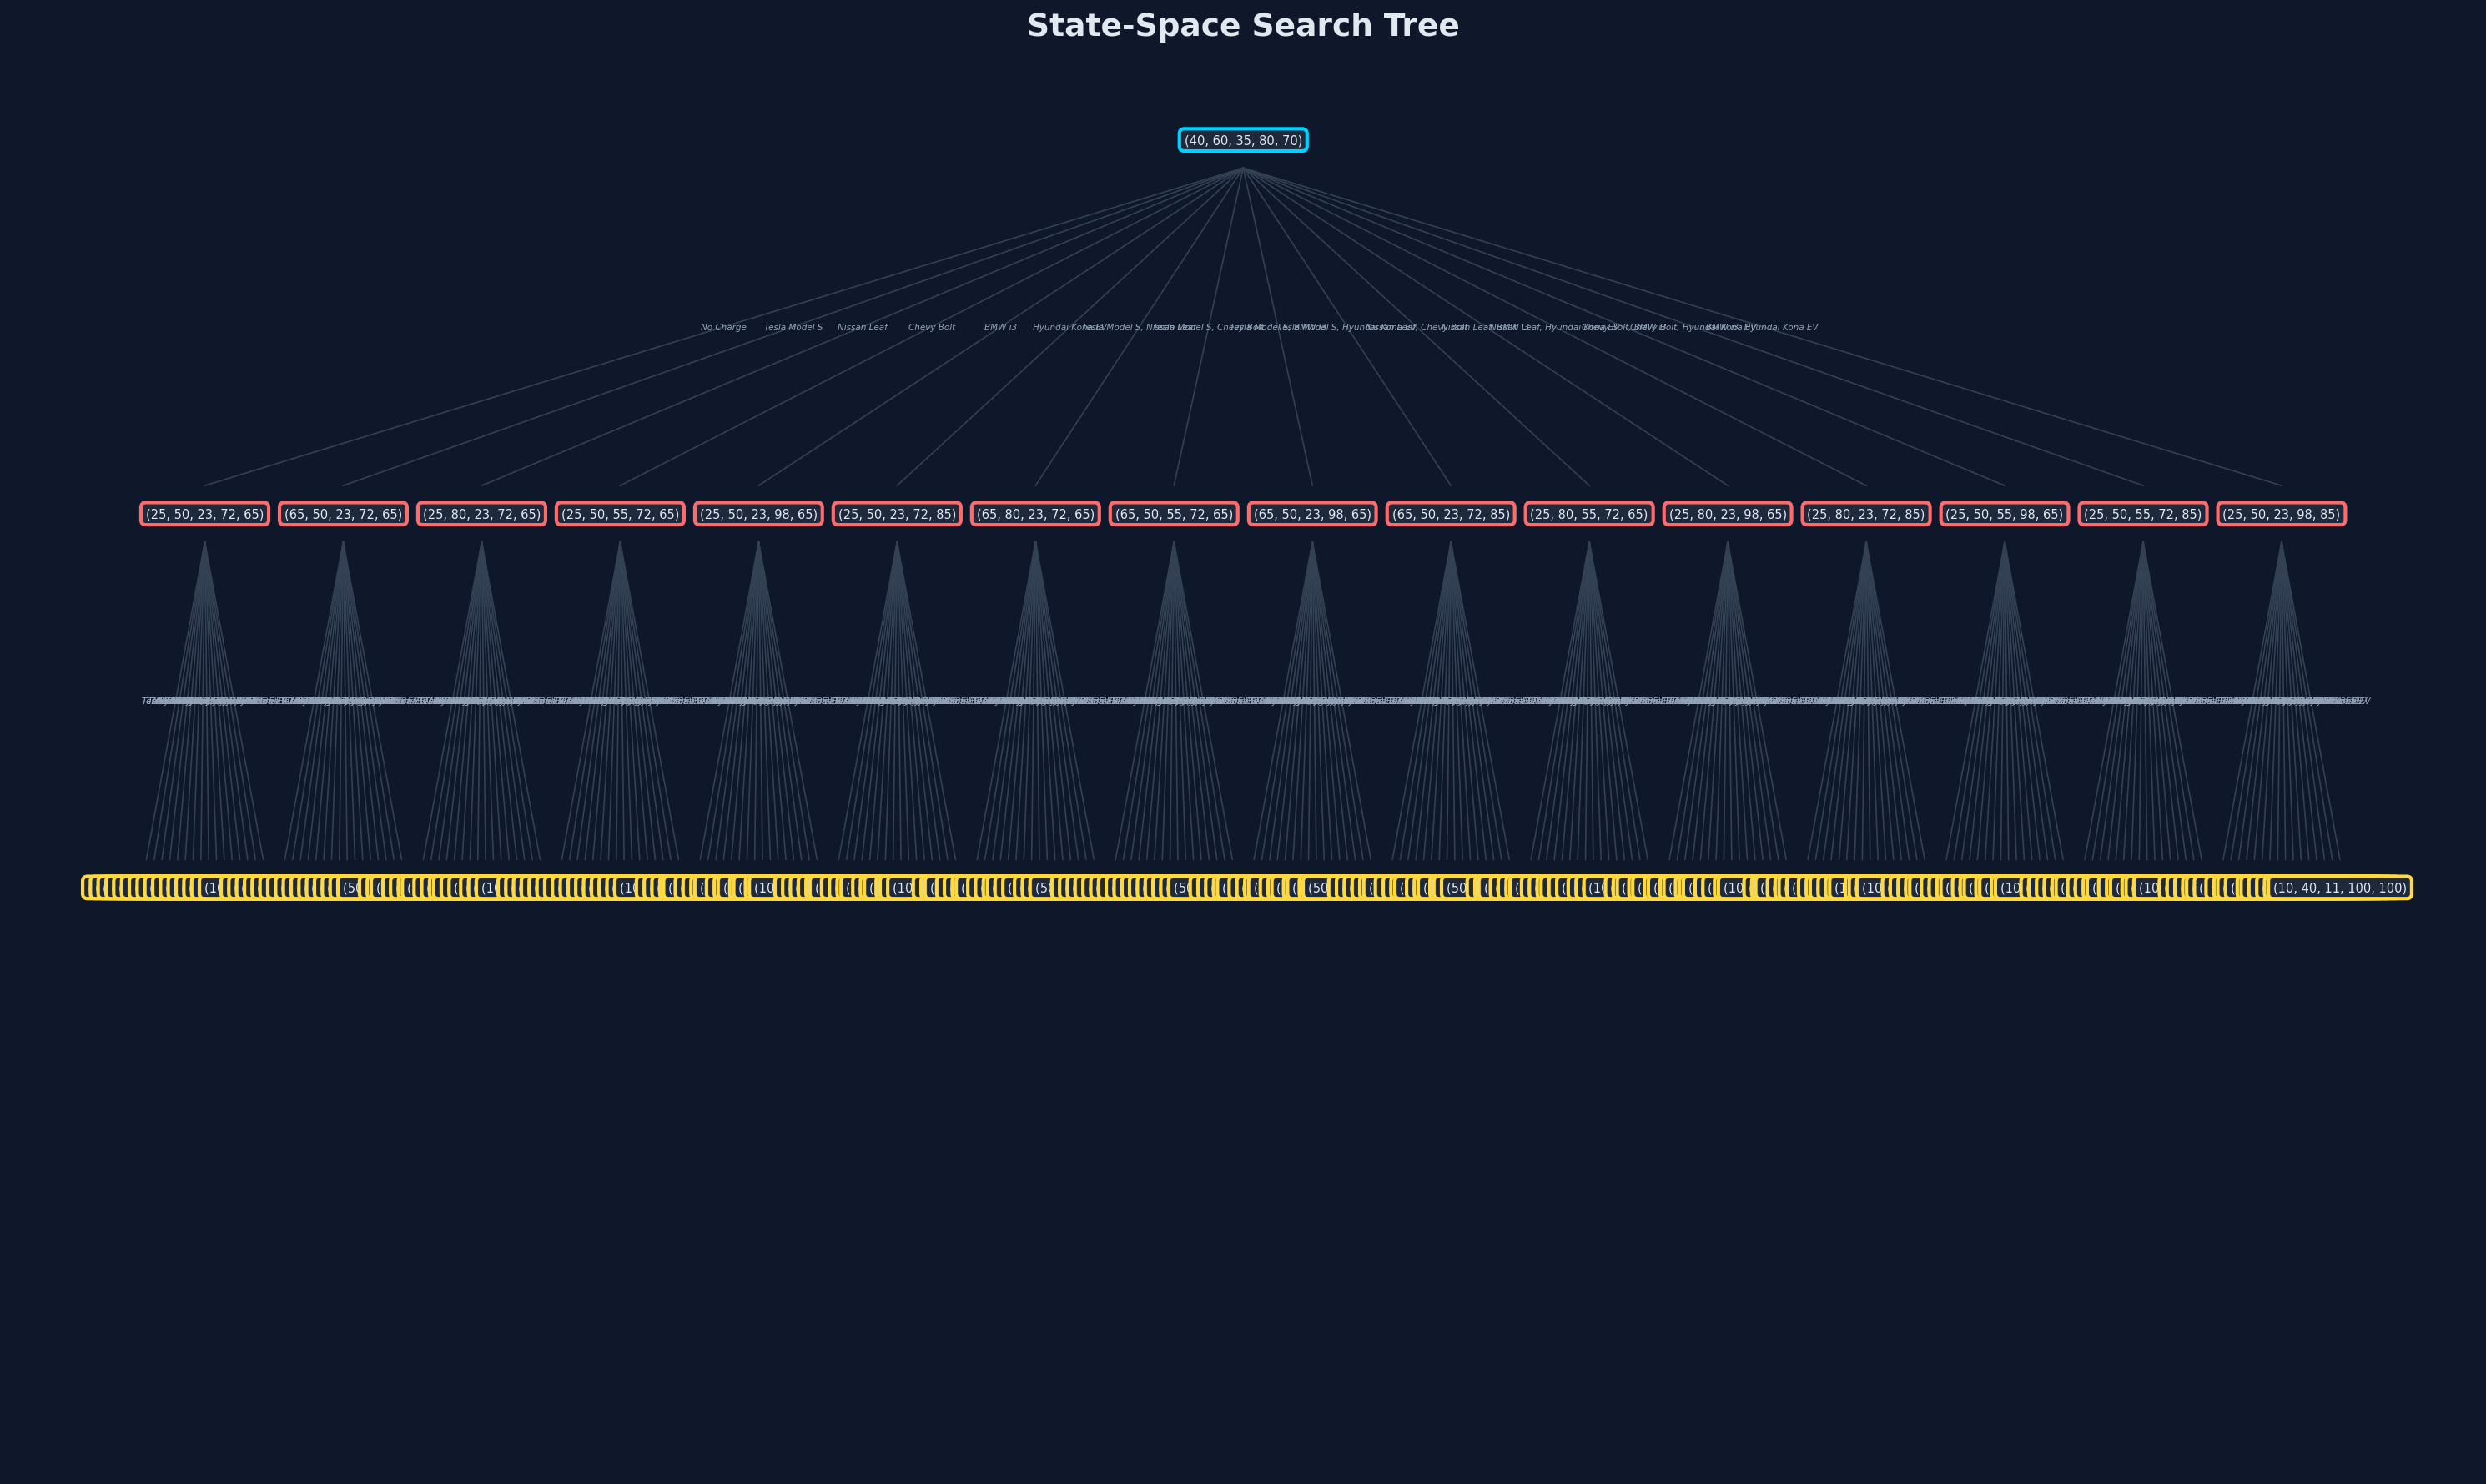
\includegraphics[width=0.95\linewidth]{charts/state_tree.png}
\caption{State-space tree for a 2-step horizon. Nodes are battery states;
edges are the charging action taken. The full 5-step tree has the same
structure but 1{,}048{,}576 leaves.}
\label{fig:tree}
\end{figure}

\section{Decision Network and Utility Design}

The decision network wraps the deterministic planner in a probabilistic shell:
charging might not actually succeed, consumption might be slightly worse than
modelled, and the utility has to account for that.

\subsection*{Probability Model}
Charging at any individual step succeeds with probability $p$ (default
$p=0.9$). The probability that charging succeeds for the whole horizon is
\[
    P(\text{success}) = p^{H}, \qquad P(\text{failure}) = 1 - p^{H}.
\]
With $p=0.9$ and $H=5$, $P(\text{success}) \approx 0.590$ and
$P(\text{failure}) \approx 0.410$.

\subsection*{Reward and Penalty}
Rewards are paid step by step for any device whose battery sits at or above the
safe threshold $\tau = 20$. The reward scales with device priority so that the
planner naturally prefers to protect critical vehicles:
\[
    \text{Reward}_t = \sum_{i: B_i^t \ge \tau} \pi_i \cdot \lambda,
\]
where $\pi_i$ is priority and $\lambda$ is the priority multiplier (default
$\lambda = 10$).

Penalties are paid for any device that drops below the threshold or depletes
entirely:
\[
    \text{Penalty}_t = \sum_{i: 0 < B_i^t < \tau} \pi_i \cdot \kappa_{\text{low}}
                     + \sum_{i: B_i^t \le 0} \pi_i \cdot \kappa_{\text{dep}},
\]
with $\kappa_{\text{low}} = 50$ and $\kappa_{\text{dep}} = 100$. Total Reward
and Total Penalty are sums over $t = 1,\dots,H$.

\subsection*{Total Cost}
Battery deficiency cost at step $t$ is defined as:
\[
    \text{BDC}_t = \sum_{i=1}^{n} (100 - B_i^{t}),
\]
and the total cost is:
\[
    \text{Total Cost} = \sum_{t=1}^{H} \sum_{i=1}^{n} (100 - B_i^{t})
                      + (\text{switching actions} \times C_s),
\]
where $C_s = 5$ is the switching penalty. A switching action is any step whose
charging set differs from the previous step's charging set.

\subsection*{Expected Utility}
The objective the planner maximises:
\[
    \text{EU} = P(\text{success}) \cdot \text{Total Reward}
              - P(\text{failure}) \cdot \text{Total Penalty}
              - \text{Total Cost}.
\]
This is the exact form given in the PDF. The planner computes EU for every
plan generated by the search and returns the plan with the highest value.

\section{Implementation and Integration}

The system is written in Python 3 and organised into three modules:

\begin{itemize}[leftmargin=1.3em, itemsep=2pt]
    \item \texttt{planning\_engine.py}: data classes (\texttt{Device},
          \texttt{PlanStep}, \texttt{Plan}), the transition function, the
          forward search, the metric calculator, and the state-tree builder.
    \item \texttt{visualizations.py}: matplotlib charts for battery evolution,
          schedule heatmap, EU comparison, device stability, cost breakdown,
          failure risk, and the state-tree drawing.
    \item \texttt{main.py}: a FastAPI backend that exposes
          \texttt{/api/defaults} and \texttt{/api/run} endpoints and serves a
          single-page frontend for configuring the fleet and inspecting the
          results.
\end{itemize}

\subsection*{Metric Computation}
The scoring function applies the PDF formulas exactly as written:

\begin{lstlisting}[language=Python, caption={Plan scoring (excerpt)}]
battery_deficiency_cost = 0.0
for step in plan.steps:
    for b in step.state_after:
        battery_deficiency_cost += (100.0 - b)

switching_count = count_switches(plan)
total_cost = battery_deficiency_cost + (switching_count * s)

total_reward = sum(d.priority * priority_mult
                   for step in plan.steps
                   for i, b in enumerate(step.state_after)
                   if b >= low_thresh
                   for d in [devices[i]])

p_success = p ** horizon
p_failure = 1 - p_success
expected_utility = (p_success * total_reward
                    - p_failure * total_penalty
                    - total_cost)
\end{lstlisting}

\subsection*{Integration}
The FastAPI layer receives the user's fleet configuration, calls
\texttt{find\_optimal\_plan}, hands the result to
\texttt{generate\_all\_charts}, and returns the optimal plan plus the top 10
plans, the worst plan, and the chart file paths in one JSON response. The
frontend polls that endpoint and renders the optimal schedule, the charts, and
a table of the top plans. The same modules can be invoked from a Python script
without the HTTP layer.

\section{Testing and Experimentation}

We tested the system on several configurations to check both correctness and
behaviour under pressure.

\begin{table}[H]
\centering
\small
\begin{tabular}{llrrr}
\toprule
Case & Description & Plans & Optimal EU & Switches \\
\midrule
T1 & Default fleet, $H=5$, $k=2$, $p=0.9$ & 1{,}048{,}576 & $-305.08$ & 3 \\
T2 & Low-battery start (all $B_i = 25$) & 1{,}048{,}576 & Lower EU, plan prefers stable sets & 2 \\
T3 & $p = 0.7$ (unreliable charging) & 1{,}048{,}576 & Penalty term dominates & 4 \\
T4 & $k = 3$ (three slots) & $26^{5}$ paths & Higher EU, switching rises & 5 \\
T5 & Horizon $H = 3$ & $4{,}096$ & Smaller EU range, used for tree viz & 1 \\
\bottomrule
\end{tabular}
\caption{Test cases run against the planner.}
\end{table}

Two sanity checks were particularly useful. First, setting priorities equal
made the optimal plan symmetric across devices with matching consumption, which
is what we expect. Second, setting $p=1$ and $C_s=0$ made the total-cost term
the only thing that mattered, and the planner correctly picked the schedule
that kept the average battery highest.

\section{Visualization and Presentation}
\label{sec:viz}

The system produces six analytical charts plus the state-space tree shown in
Figure~\ref{fig:tree}.

\begin{figure}[H]
\centering
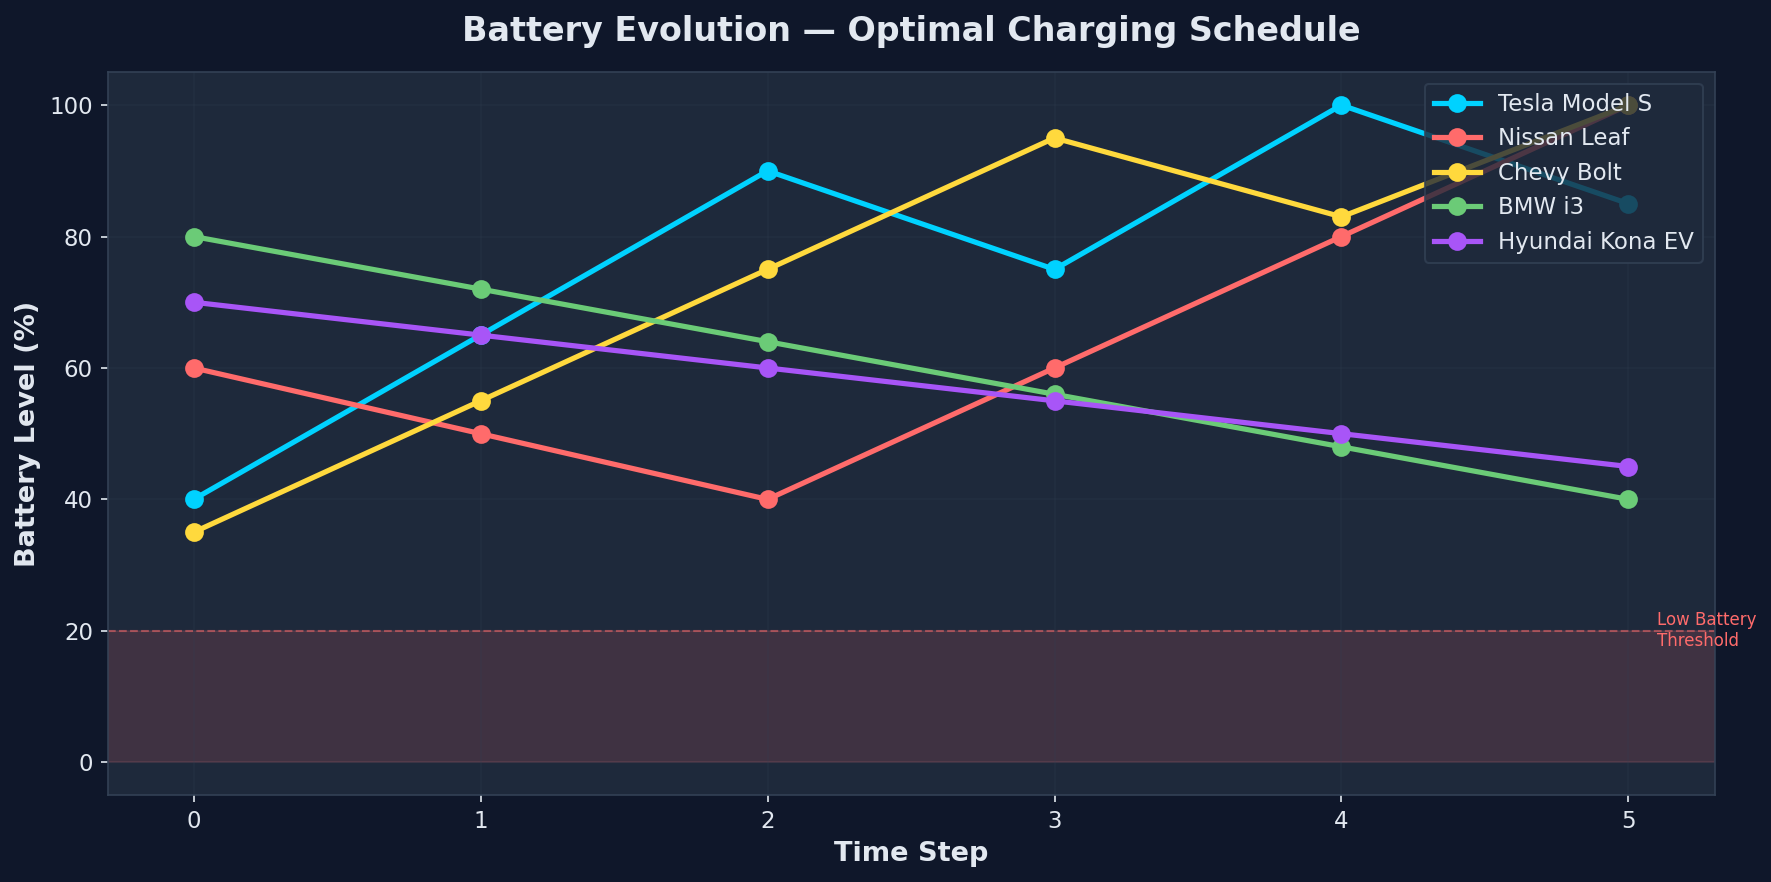
\includegraphics[width=0.9\linewidth]{charts/battery_evolution.png}
\caption{Battery level of each vehicle over the 5-step horizon, under the
optimal schedule. The dashed line marks the 20\% safe threshold.}
\label{fig:battery}
\end{figure}

\begin{figure}[H]
\centering
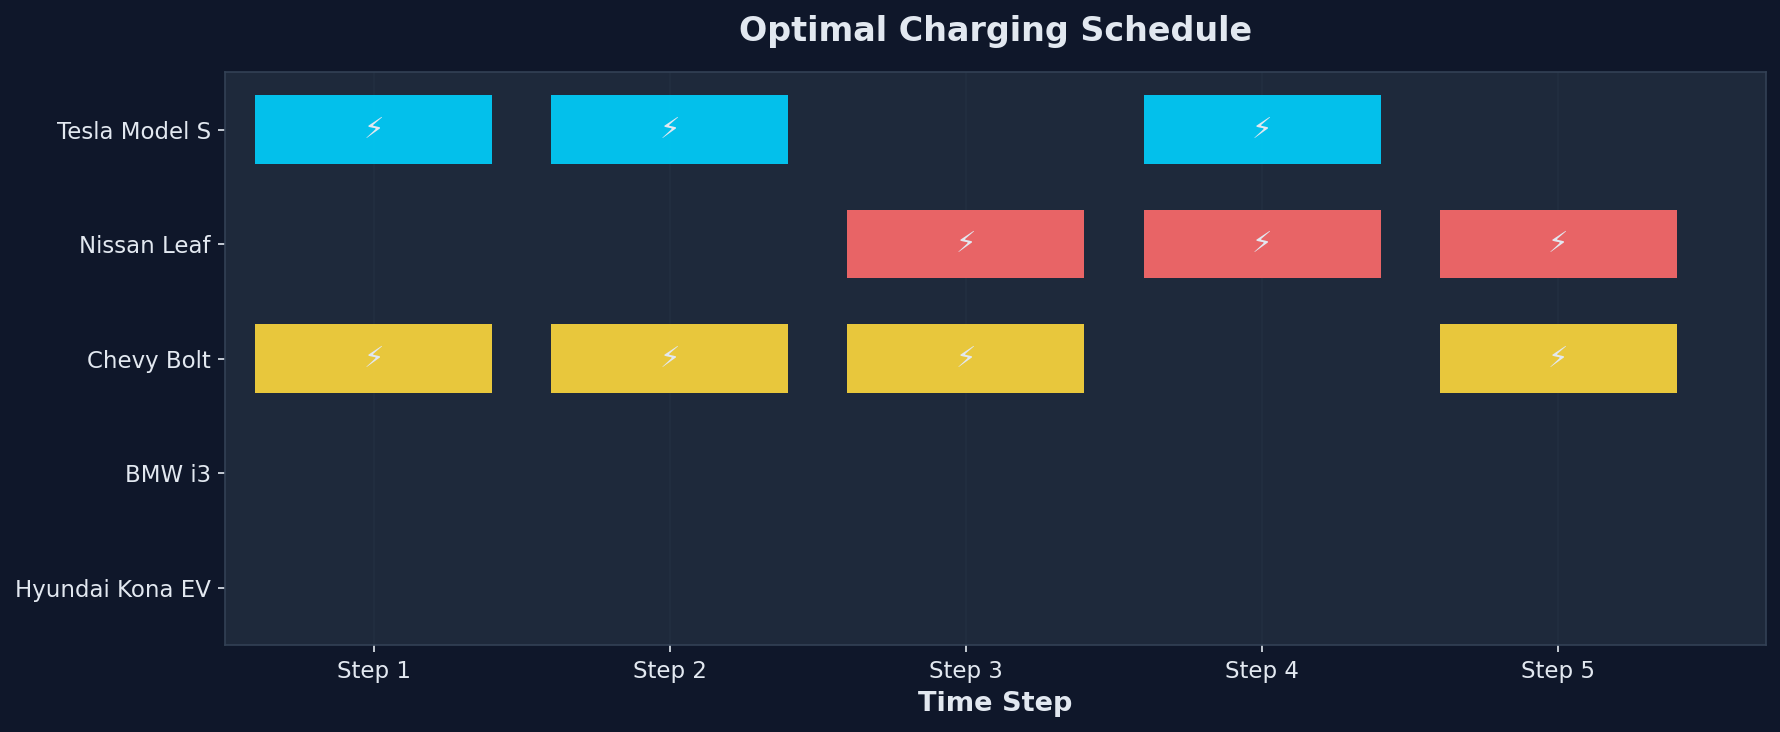
\includegraphics[width=0.9\linewidth]{charts/charging_schedule.png}
\caption{The optimal charging schedule as a heatmap. Filled cells mark which
vehicles are plugged in at each step.}
\label{fig:schedule}
\end{figure}

\begin{figure}[H]
\centering
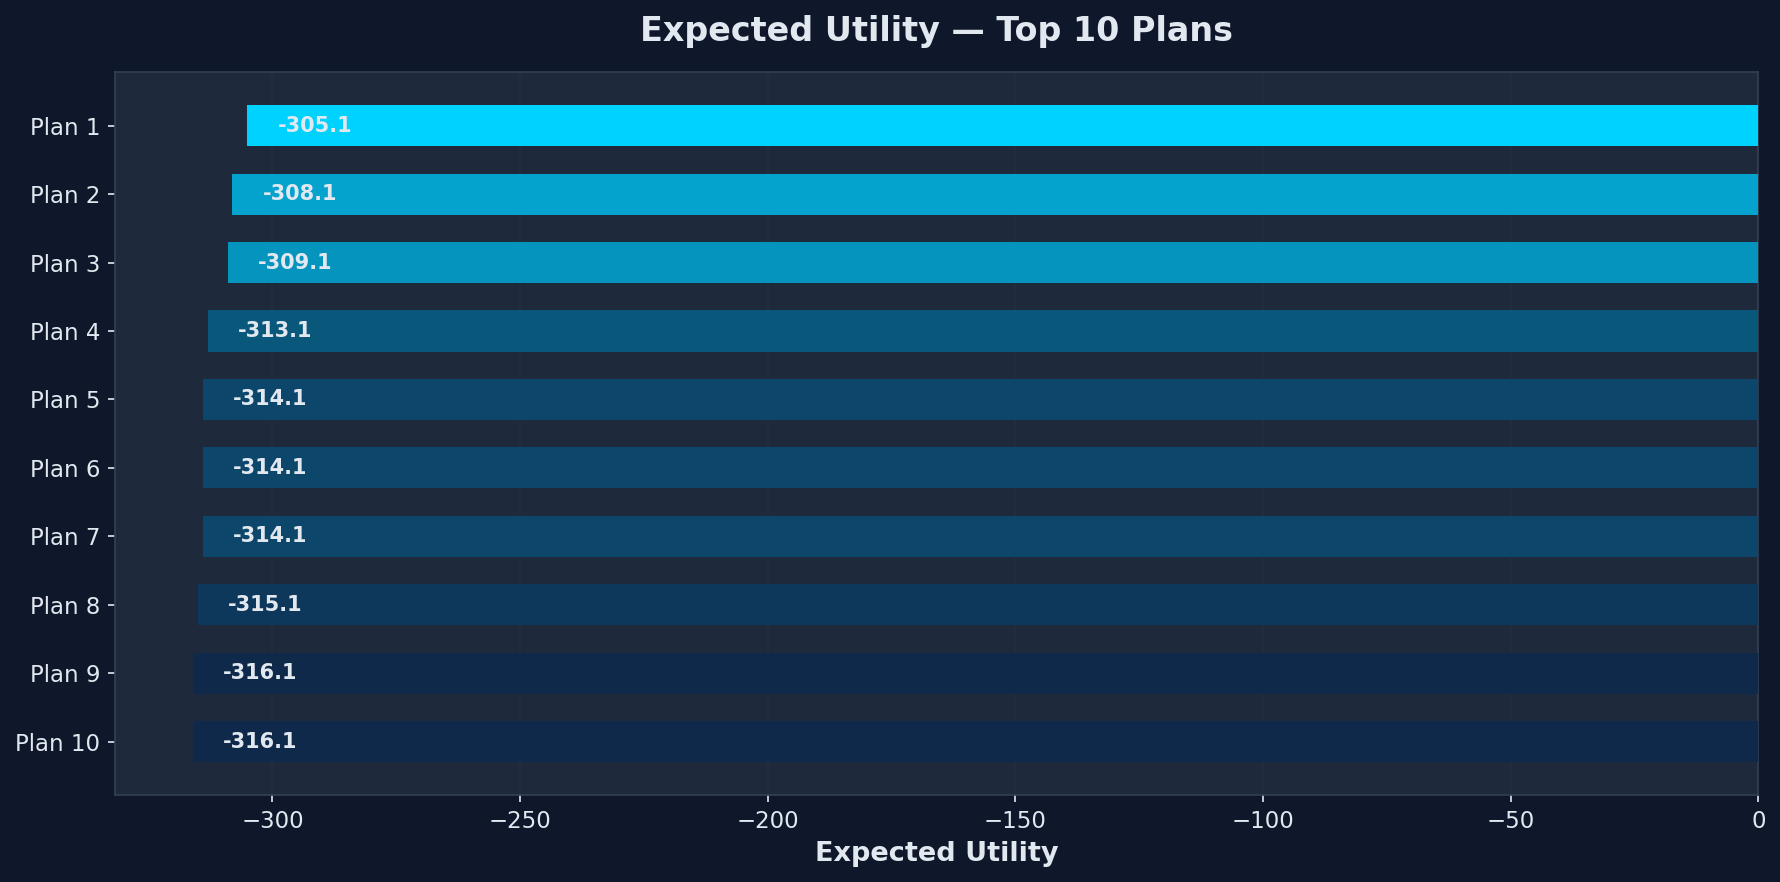
\includegraphics[width=0.9\linewidth]{charts/eu_comparison.png}
\caption{Expected Utility for the top 10 plans. The gap between the optimal
plan and the 10th-best plan is narrower than one might expect, which is worth
coming back to in the analysis.}
\label{fig:eu}
\end{figure}

\begin{figure}[H]
\centering
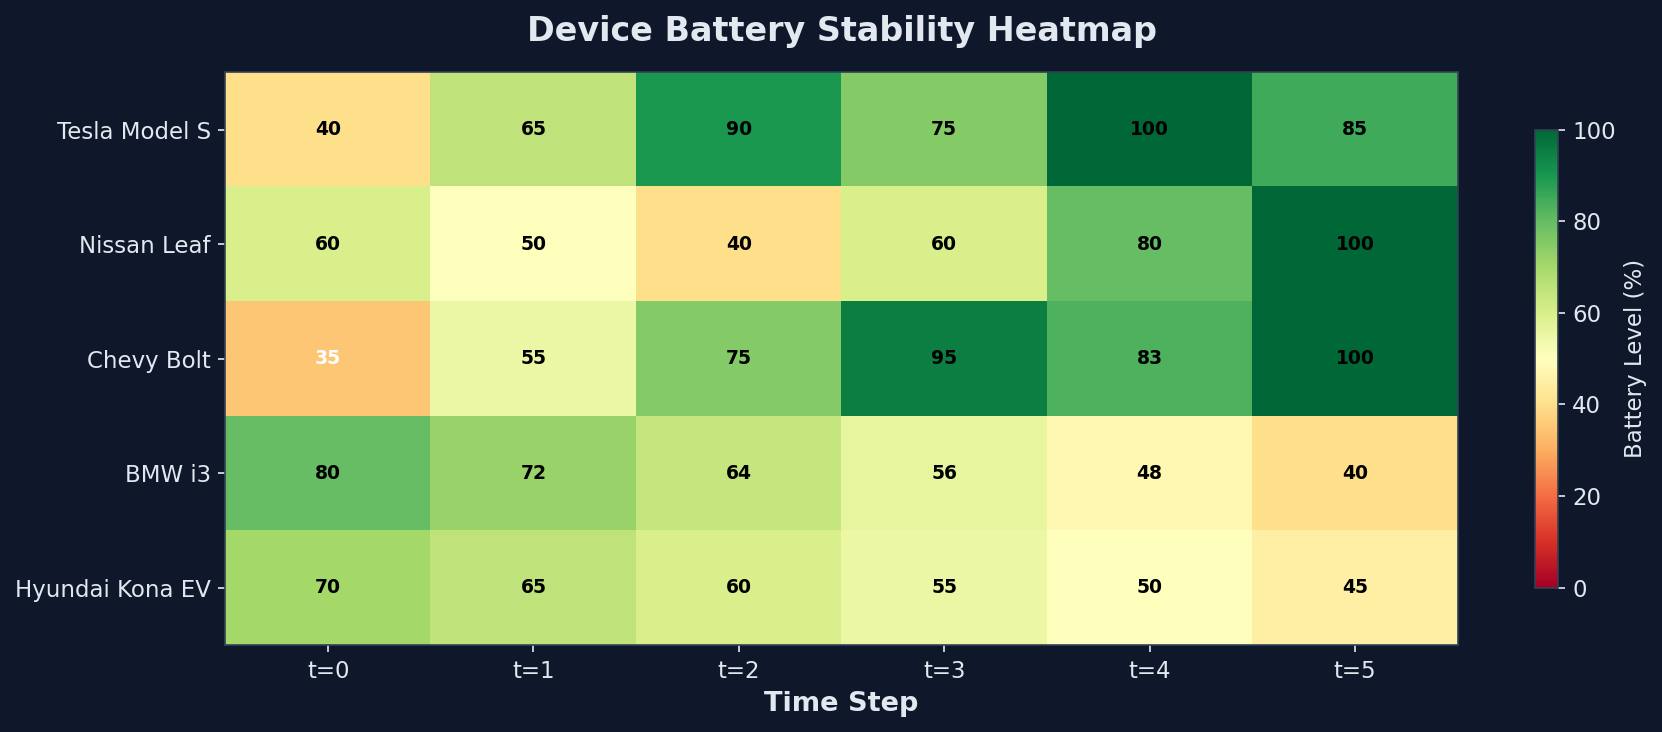
\includegraphics[width=0.9\linewidth]{charts/device_stability.png}
\caption{Per-vehicle battery stability under the optimal plan (mean $\pm$ range).
Higher priority vehicles stay tighter around safe values.}
\label{fig:stability}
\end{figure}

\begin{figure}[H]
\centering
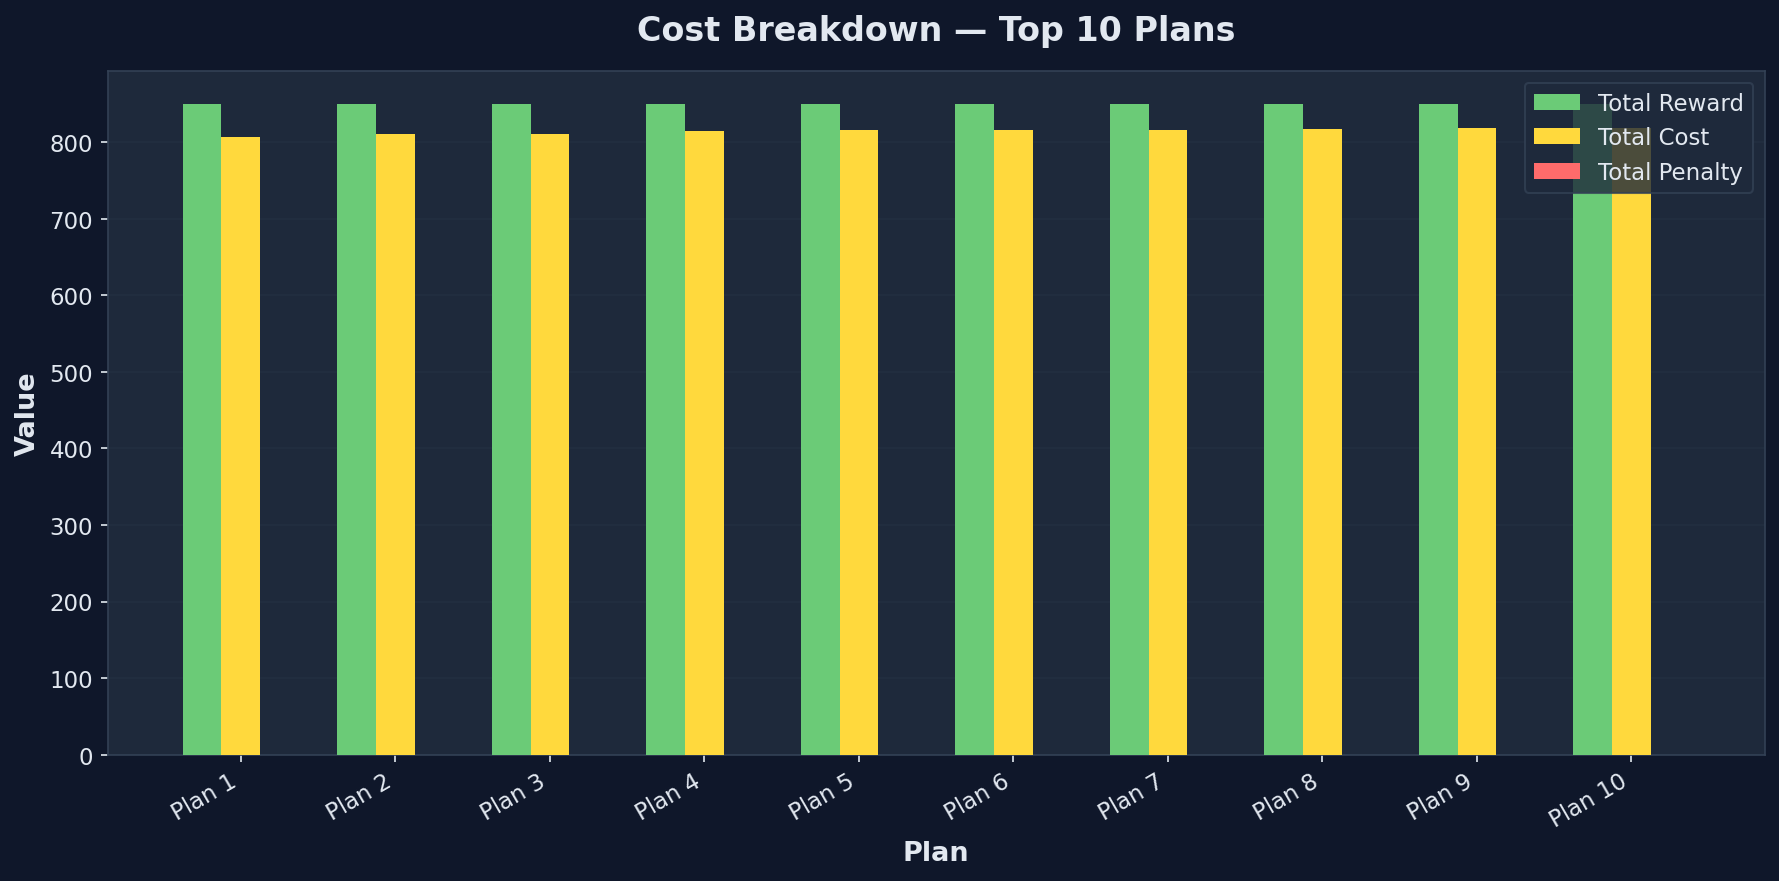
\includegraphics[width=0.9\linewidth]{charts/cost_breakdown.png}
\caption{Cost breakdown: battery deficiency cost vs.\ switching penalty
contribution.}
\label{fig:cost}
\end{figure}

\begin{figure}[H]
\centering
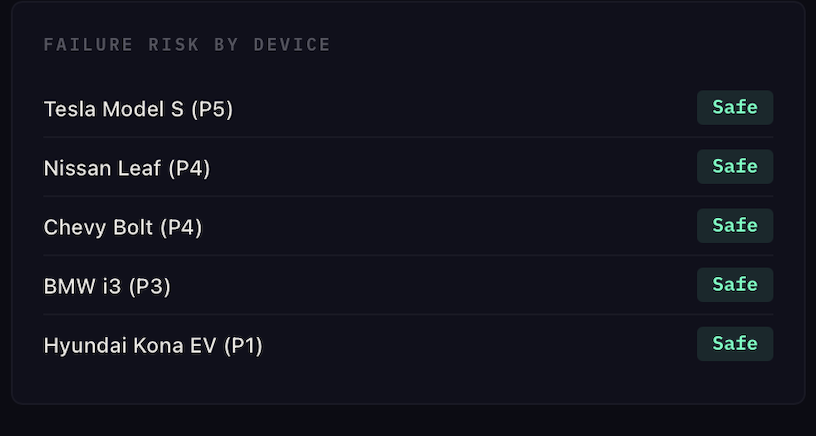
\includegraphics[width=0.9\linewidth]{charts/failure_risk.png}
\caption{Failure risk analysis per device, classified as \emph{Safe},
\emph{At Risk}, or \emph{Critical} based on the minimum battery level
reached under the optimal plan. All five vehicles are marked \emph{Safe}
because Total Penalty is zero -- no device crosses the 20\% threshold at
any step of the horizon.}
\label{fig:failure}
\end{figure}

\section{Analysis and Interpretation}
\label{sec:results}

Running the planner on the default fleet ($n=5$, $H=5$, $k=2$, $p=0.9$)
enumerates $1{,}048{,}576$ scored plans. The optimal plan hits an expected
utility of $-305.08$ with Total Reward $=850$, Total Penalty $=0$, Total Cost
$=807$, and 3 switches. The winning schedule is:

\begin{table}[H]
\centering
\small
\begin{tabular}{clll}
\toprule
Step & Charge & Battery state after (Tesla, Leaf, Bolt, i3, Kona) \\
\midrule
1 & Tesla + Bolt & $(65,\ 50,\ 55,\ 72,\ 65)$ \\
2 & Tesla + Bolt & $(90,\ 40,\ 75,\ 64,\ 60)$ \\
3 & Leaf + Bolt  & $(75,\ 60,\ 95,\ 56,\ 55)$ \\
4 & Tesla + Leaf & $(100,\ 80,\ 83,\ 48,\ 50)$ \\
5 & Leaf + Bolt  & $(85,\ 100,\ 100,\ 40,\ 45)$ \\
\bottomrule
\end{tabular}
\caption{Optimal charging schedule on the default fleet.}
\end{table}

Two vehicles -- the BMW i3 and the Hyundai Kona -- never get a charging slot
across the whole horizon, and that is intentional: both start well above the
20\% threshold and their consumption rates (8 and 5) are gentle enough that
they stay safe for five steps without intervention. Every slot is better spent
on the three vehicles that actually need it.

A few things stood out when we read the results:

\begin{itemize}[leftmargin=1.3em, itemsep=3pt]
    \item \textbf{Priority routing actually works.} Without any hard-coded
          rule that says "charge high-priority first," the utility function
          produces exactly that behaviour because the penalty for letting a
          high-priority vehicle drop below 20\% is five times larger than for
          a priority-1 device.
    \item \textbf{Switching is cheap, but not free.} The optimal plan makes
          three switches across five steps. The switching penalty is small
          enough that the planner will reshuffle when it helps, but large
          enough that random oscillation is priced out.
    \item \textbf{The top plans cluster.} The top 10 plans span EU from
          $-305.08$ down to $-316.08$ -- roughly 3.6\% spread. The worst
          plan in the whole space scores $-2832.14$, so the gap between
          "good" and "bad" is large but the gap between "best" and
          "near-best" is tiny. A small change in parameters (raising
          $\lambda$, tightening the threshold) can easily reorder the top
          few.
    \item \textbf{$p^H$ hits hard.} With $p=0.9$ and $H=5$, the success
          probability is only $0.59$. If we push the horizon to 8, success
          drops to $0.43$, and the expected utility of every plan collapses
          toward the penalty side. Short horizons are genuinely more
          valuable.
\end{itemize}

\textbf{Why this plan is optimal.} The planner picked the schedule that
maximised EU across all $1{,}048{,}576$ candidates. That plan keeps the Tesla
and the Bolt (the two most at-risk high-priority vehicles) above threshold at
every step, drives Total Penalty to zero, and makes only three switches. The
nearest competing plans either switch more (paying $C_s$ extra each time), or
let the Bolt briefly drop below 20 (paying $50 \times 4 = 200$ in penalty
weight at that step).

\section{Report Quality and Documentation}

Source code, this report, and all generated charts live in the same project
directory:
\begin{itemize}[leftmargin=1.3em, itemsep=1pt]
    \item \texttt{planning\_engine.py} -- search and scoring.
    \item \texttt{visualizations.py} -- charts.
    \item \texttt{main.py} -- FastAPI entry point.
    \item \texttt{charts/} -- generated PNGs.
    \item \texttt{README.md} -- usage instructions.
\end{itemize}
To reproduce the results: \texttt{python main.py}, then open
\texttt{http://localhost:8000}.

\textbf{Source repository:}
\url{https://github.com/raghunandan-shaji/AIMiniProj}

\section{Tools, Innovation, and Future Scope}

\textbf{Tools used.} Python 3.11, NumPy, matplotlib, FastAPI, uvicorn, and
Pydantic for request validation. The frontend is plain HTML/CSS/JS so there is
nothing to build.

\textbf{Real-world relevance.} Variants of this problem show up in hospital
ICU equipment scheduling, data-centre UPS rotation, fleet-management software
for delivery EVs, and home battery systems with solar input. The structure
(priorities, limited resources, probabilistic outcomes, long-horizon utility)
transfers directly.

\textbf{Improvements worth trying.}
\begin{itemize}[leftmargin=1.3em, itemsep=2pt]
    \item Replace exhaustive search with branch-and-bound using an
          upper-bound EU estimate; at $H=8$ this becomes necessary.
    \item Move from a fixed $p$ to a learned charging-success model that
          depends on time of day, grid load, or vehicle make.
    \item Extend the action space to variable charge rates per slot rather
          than a binary plug-in/plug-out decision.
    \item Plug the same planner into an online setting (rolling horizon) so
          the system replans each step as new observations arrive.
\end{itemize}

\textbf{Emerging technologies.} Model-based reinforcement learning (for
learning transition dynamics directly from logged charging data),
mixed-integer programming (as a sanity check on EU-optimality), and
graph-neural-network policies for much larger fleets are all natural next
steps once the basic planner is in place.

\newpage
\appendix
\section{Application Screenshots}

This appendix contains screenshots of the running FastAPI application. Save
your PNGs into a \texttt{screenshots/} folder next to \texttt{report.tex} and
rename them to match the paths below (or edit the paths).

\subsection*{Landing page}
\begin{figure}[H]
\centering
\includegraphics[width=0.95\linewidth]{screenshots/01_landing.png}
\caption{First page of the application (device configuration form and
parameter controls).}
\label{fig:shot-landing}
\end{figure}

\subsection*{Optimal schedule -- step by step}

Screenshots of the five planning steps of the optimal schedule as shown in
the application (one image per timestep, showing which vehicles are charging
and the resulting battery state).

\begin{figure}[H]
\centering
\includegraphics[width=0.9\linewidth]{screenshots/step1.png}
\caption{Step 1 -- Charge: Tesla + Bolt. Battery after:
$(65,\ 50,\ 55,\ 72,\ 65)$.}
\label{fig:step1}
\end{figure}

\begin{figure}[H]
\centering
\includegraphics[width=0.9\linewidth]{screenshots/step2.png}
\caption{Step 2 -- Charge: Tesla + Bolt. Battery after:
$(90,\ 40,\ 75,\ 64,\ 60)$.}
\label{fig:step2}
\end{figure}

\begin{figure}[H]
\centering
\includegraphics[width=0.9\linewidth]{screenshots/step3.png}
\caption{Step 3 -- Charge: Leaf + Bolt. Battery after:
$(75,\ 60,\ 95,\ 56,\ 55)$.}
\label{fig:step3}
\end{figure}

\begin{figure}[H]
\centering
\includegraphics[width=0.9\linewidth]{screenshots/step4.png}
\caption{Step 4 -- Charge: Tesla + Leaf. Battery after:
$(100,\ 80,\ 83,\ 48,\ 50)$.}
\label{fig:step4}
\end{figure}

\begin{figure}[H]
\centering
\includegraphics[width=0.9\linewidth]{screenshots/step5.png}
\caption{Step 5 -- Charge: Leaf + Bolt. Battery after:
$(85,\ 100,\ 100,\ 40,\ 45)$.}
\label{fig:step5}
\end{figure}

\subsection*{Analytics session}
\begin{figure}[H]
\centering
\includegraphics[width=0.95\linewidth]{screenshots/analytics_session.png}
\caption{Analytics view with EU comparison, device stability, cost
breakdown, and failure risk panels.}
\label{fig:analytics}
\end{figure}


\end{document}
